\documentclass[12pt,a4paper]{report}

\usepackage[utf8]{inputenc}
\usepackage[T1]{fontenc}
\usepackage[french]{babel}
\usepackage{geometry}
\usepackage{setspace}
\usepackage{graphicx}
\usepackage{float}
\usepackage{booktabs}
\usepackage{longtable}
\usepackage{array}
\usepackage{xcolor}
\usepackage{hyperref}
\usepackage{titlesec}
\usepackage{fancyhdr}
\usepackage{listings}
\usepackage{caption}
\usepackage{enumitem}

\geometry{margin=2.2cm}
\setstretch{1.15}
\setlength{\emergencystretch}{3em}

\definecolor{rougeprincipal}{RGB}{190,30,45}
\definecolor{bleufonce}{RGB}{20,35,60}
\definecolor{grisclair}{RGB}{246,247,249}

\hypersetup{colorlinks=true, linkcolor=bleufonce, urlcolor=rougeprincipal, pdftitle={Systeme Intelligent de Maintenance Predictive}}

\titleformat{\chapter}[display]{\normalfont\huge\bfseries\color{bleufonce}}{\chaptertitlename\ \thechapter}{8pt}{\Huge}
\titleformat{\section}{\normalfont\Large\bfseries\color{bleufonce}}{\thesection}{0.8em}{}
\titleformat{\subsection}{\normalfont\large\bfseries\color{rougeprincipal}}{\thesubsection}{0.8em}{}
\titlespacing*{\chapter}{0pt}{-8pt}{18pt}

\pagestyle{fancy}
\fancyhf{}
\lhead{Maintenance Predictive Intelligence}
\rhead{Rapport Technique}
\cfoot{\thepage}

\lstset{basicstyle=\ttfamily\small, keywordstyle=\color{bleufonce}\bfseries, stringstyle=\color{rougeprincipal}, commentstyle=\color{gray}, breaklines=true, frame=single, backgroundcolor=\color{grisclair}, columns=fullflexible, captionpos=b}
\setlist[itemize]{topsep=4pt,itemsep=2pt,parsep=1pt}

\begin{document}

\begin{titlepage}
    \centering
    \vspace*{0.8cm}
    {\Large\textbf{Rapport de Projet}}\\[0.25cm]
    {\large\color{rougeprincipal}\textbf{Intelligence Artificielle Industrielle}}\\[1.1cm]
    \rule{0.82\textwidth}{0.8pt}\\[0.55cm]
    {\Huge\textbf{Système Intelligent de Maintenance Prédictive}}\\[0.45cm]
    {\Large\textbf{Prédiction des défaillances machines par Machine Learning}}\\[0.55cm]
    \rule{0.82\textwidth}{0.8pt}\\[1.2cm]
    \begin{minipage}{0.82\textwidth}
        \centering
        \large
        Ce rapport présente la problématique industrielle, la solution proposée, le pipeline de données, l'entraînement, l'évaluation, l'API, le dashboard, le ML Lab, le déploiement Railway et les résultats opérationnels du système.
    \end{minipage}
    \vfill
    \begin{minipage}{0.72\textwidth}
        \large
        \begin{tabular}{@{}p{0.35\textwidth}p{0.55\textwidth}@{}}
            \textbf{Réalisé par :} & Mohamed Aziz Mansour \\
                                   & Rimel Zouari \\
                                   & Mohamed Ncib \\[0.45cm]
            \textbf{Domaine :} & Machine Learning, Deep Learning, IoT industriel \\[0.2cm]
            \textbf{Modèle actif :} & GradientBoosting \\[0.2cm]
            \textbf{Seuil API :} & 0.25 \\
        \end{tabular}
    \end{minipage}
    \vfill
    {\large Année universitaire 2025--2026}\\[0.4cm]
\end{titlepage}

\pagenumbering{roman}
\chapter*{Résumé}
Ce projet réalise un système complet de maintenance prédictive pour anticiper les pannes de machines industrielles. Le travail part de fichiers CSV bruts, effectue la découverte des données, fusionne les sources, nettoie les incohérences, construit des variables explicables, entraîne plusieurs modèles, sélectionne un modèle actif, expose les prédictions via FastAPI et affiche le résultat dans un frontend synchronisé.

La difficulté principale vient du déséquilibre des classes : après nettoyage, seulement 3.48\% des observations correspondent à une panne. Une accuracy brute peut donc être trompeuse. Le projet utilise des métriques adaptées : balanced accuracy, précision, recall, F1, ROC AUC, matrice de confusion et taux d'alerte. Le modèle actif est GradientBoosting avec un seuil de production de 0.25. Il atteint 89.05\% de balanced accuracy, 85.94\% de précision, 78.57\% de pannes capturées et 3.20\% de taux d'alerte.

\tableofcontents
\listoffigures
\listoftables
\clearpage
\pagenumbering{arabic}

\chapter{Problématique et Solution}

\section{Contexte industriel}
Les machines industrielles fonctionnent sous des contraintes variables : température, couple, vitesse, usure d'outil et charge mécanique. Une panne imprévue peut arrêter une ligne de production, augmenter les coûts, réduire la qualité et créer un risque de sécurité. La maintenance corrective attend la panne, tandis que la maintenance préventive intervient selon un calendrier fixe. Ces deux approches ne tiennent pas suffisamment compte de l'état réel de la machine.

La maintenance prédictive répond à ce besoin en utilisant les données pour anticiper les défaillances. Le but n'est pas seulement de produire un score de modèle, mais de donner une décision exploitable : continuer la surveillance, planifier une inspection ou inspecter immédiatement.

\section{Problème de classes déséquilibrées}
Le dataset final contient 10 000 lignes, dont seulement 348 pannes. Cela signifie que 96.52\% des cas sont normaux. Un modèle qui prédit toujours « pas de panne » semble très bon en accuracy, mais il est inutile. Le projet évite ce piège avec la balanced accuracy, la précision, le recall et la matrice de confusion.

\begin{figure}[H]
    \centering
    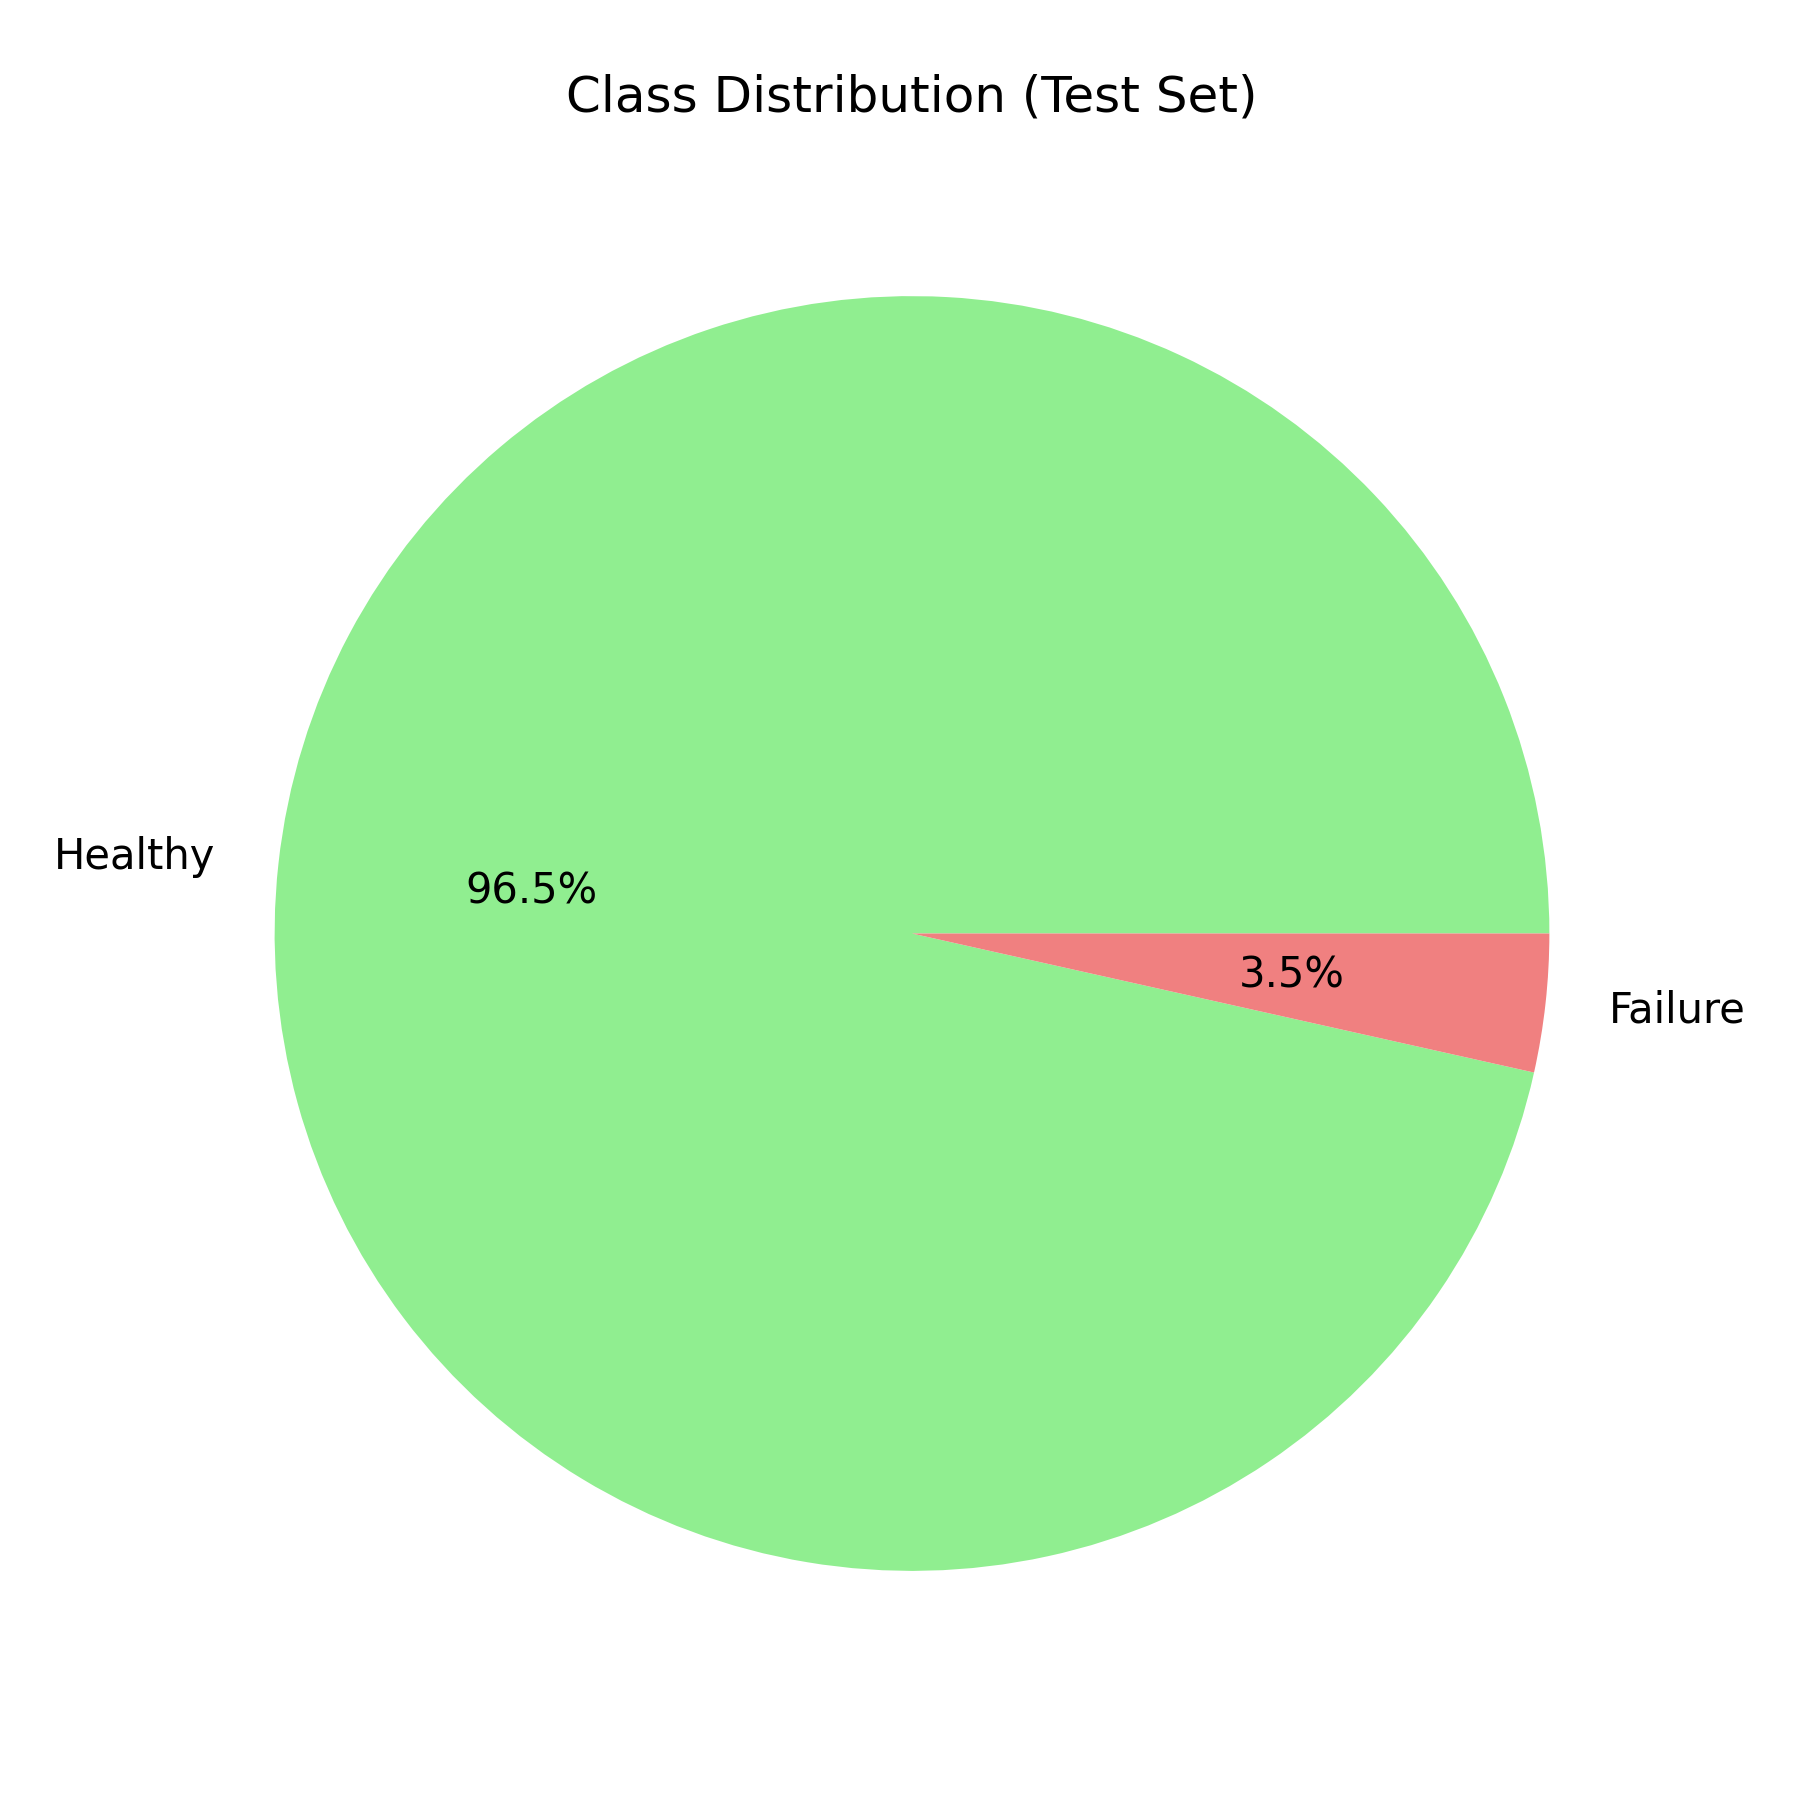
\includegraphics[width=0.78\textwidth]{assets/class_distribution.png}
    \caption{Distribution des classes après nettoyage.}
\end{figure}

\section{Solution proposée}
La solution est organisée en quatre couches :
\begin{itemize}
    \item un pipeline de données pour découvrir, nettoyer, transformer et exporter les informations ;
    \item une couche Machine Learning pour entraîner, comparer et sauvegarder les modèles ;
    \item une API FastAPI pour servir les prédictions et les données dashboard ;
    \item un frontend clair composé du dashboard, du ML Lab, de la présentation et de la page rapport.
\end{itemize}

L'utilisateur saisit les conditions de la machine. Le backend reconstruit les variables d'ingénierie, charge le modèle actif, calcule la probabilité de panne, applique le seuil 0.25 et retourne le niveau de risque ainsi que l'action recommandée.

\chapter{Données, ETL et Nettoyage}

\section{Sources brutes}
Deux fichiers bruts sont utilisés : \texttt{machine\_predictive\_maintenance.csv} et \texttt{ai4i\_2020\_predictive\_maintenance.csv}. Chaque fichier contient 10 000 observations. Les deux sources décrivent la même population de machines, mais avec des colonnes et des labels différents.

Les variables principales sont : type de produit, température de l'air, température du processus, vitesse de rotation, couple, usure de l'outil et indicateurs de panne.

\section{Fusion canonique}
Les deux fichiers ne sont pas empilés, car cela créerait des doublons et un risque de fuite de données. Ils sont fusionnés sur des clés stables : UDI, product id, type de produit, températures, vitesse, couple et usure. Les colonnes sont ensuite renommées dans un schema clair : \texttt{air\_temp\_k}, \texttt{process\_temp\_k}, \texttt{rotational\_speed\_rpm}, \texttt{torque\_nm}, \texttt{tool\_wear\_min}, \texttt{machine\_failure}.

\section{Résultats du nettoyage}
Après nettoyage, le dataset contient 10 000 lignes et 17 colonnes. Les incohérences restantes sont nulles. La répartition des familles de pannes est la suivante :

\begin{table}[H]
\centering
\begin{tabular}{lr}
\toprule
\textbf{Famille de panne} & \textbf{Nombre de lignes} \\
\midrule
No Failure & 9 652 \\
Heat Dissipation Failure & 112 \\
Power Failure & 95 \\
Overstrain Failure & 78 \\
Tool Wear Failure & 45 \\
Random Failures & 18 \\
\bottomrule
\end{tabular}
\caption{Répartition des pannes après nettoyage.}
\end{table}

\section{Séparation train, validation et test}
La séparation est stratifiée pour conserver le taux de panne dans chaque partition. Le train contient 6 000 lignes, la validation 2 000 lignes et le test 2 000 lignes. Les taux de panne restent proches de 3.5\%.

\begin{table}[H]
\centering
\begin{tabular}{lrr}
\toprule
\textbf{Jeu} & \textbf{Lignes} & \textbf{Taux de panne} \\
\midrule
Train & 6 000 & 3.483\% \\
Validation & 2 000 & 3.450\% \\
Test & 2 000 & 3.500\% \\
\bottomrule
\end{tabular}
\caption{Séparation stratifiée des données.}
\end{table}

\chapter{Feature Engineering}

\section{Objectif}
Le feature engineering transforme les mesures brutes en variables plus informatives. Les variables construites restent interprétables pour un contexte industriel : stress thermique, charge mécanique, usure, couple élevé et faible vitesse.

\section{Variables finales}
Le modèle utilise 16 variables : 13 numériques et 3 catégorielles. Les principales variables construites sont :

\begin{longtable}{p{0.28\textwidth}p{0.28\textwidth}p{0.34\textwidth}}
\toprule
\textbf{Variable} & \textbf{Formule / règle} & \textbf{Sens métier} \\
\midrule
\texttt{temp\_delta\_k} & process temp - air temp & Écart thermique. \\
\texttt{power\_proxy} & vitesse $\times$ couple & Charge mécanique approximée. \\
\texttt{torque\_speed\_ratio} & couple / vitesse & Stress à faible vitesse. \\
\texttt{thermal\_load} & delta temp $\times$ couple & Charge thermique et mécanique. \\
\texttt{wear\_temp\_stress} & usure $\times$ delta temp & Outil usé sous chaleur. \\
\texttt{high\_torque\_flag} & couple $\geq 55$ & Indicateur de couple élevé. \\
\texttt{low\_speed\_flag} & vitesse $\leq 1400$ & Indicateur de faible vitesse. \\
\texttt{wear\_risk\_band} & usure catégorisée & fresh, moderate, elevated, critical. \\
\bottomrule
\caption{Variables construites principales.}
\end{longtable}

\section{Analyse de corrélation}
\begin{figure}[H]
    \centering
    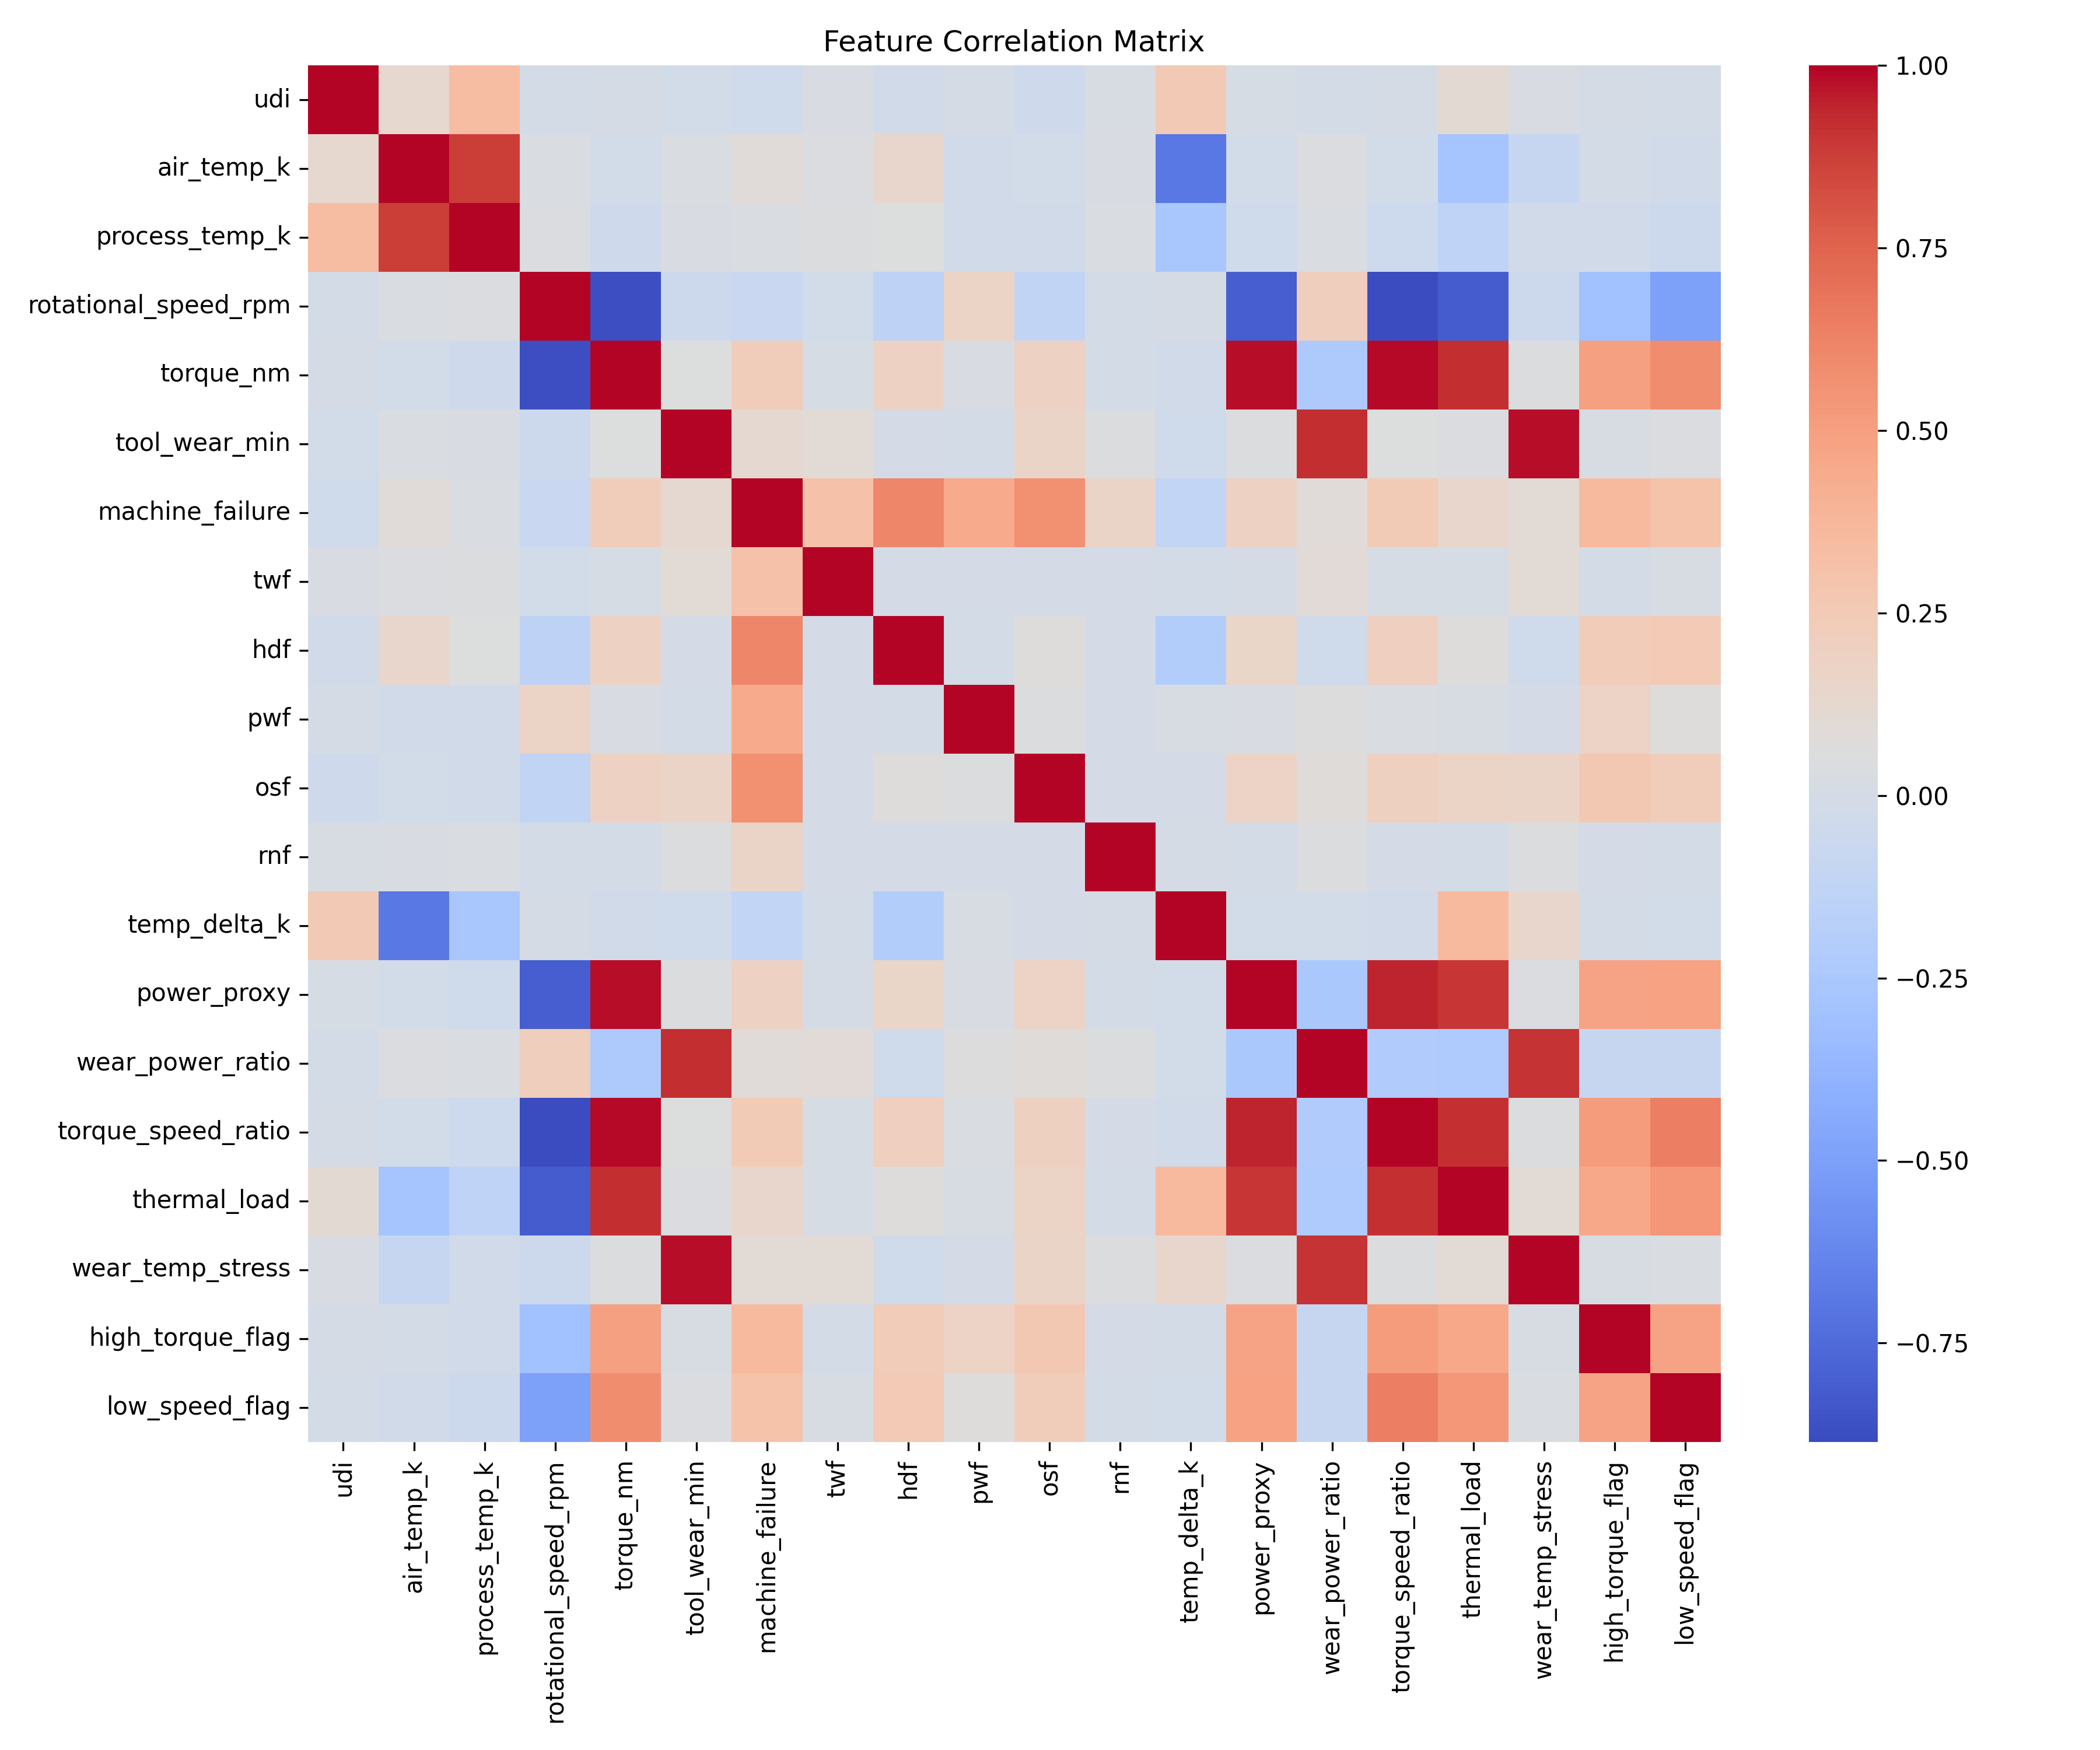
\includegraphics[width=0.88\textwidth]{assets/correlation_matrix.png}
    \caption{Matrice de corrélation des variables.}
\end{figure}

La matrice montre les relations entre variables, notamment les interactions entre vitesse, couple et température. Ces interactions justifient l'utilisation de modèles d'arbres, capables de capturer des effets non linéaires.

\chapter{Modélisation et Sélection}

\section{Modèles comparés}
Le pipeline compare LogisticRegression, RandomForest, ExtraTrees, GradientBoosting, NeuralNetwork\_MLP et DeepLearning\_TF. Les modèles classiques utilisent un pipeline de preprocessing : imputation, standardisation des variables numériques et encodage one-hot des variables catégorielles.

\section{Leaderboard}
\begin{table}[H]
\centering
\small
\begin{tabular}{lrrrrr}
\toprule
\textbf{Modèle} & \textbf{Seuil} & \textbf{Val. BA} & \textbf{Test BA} & \textbf{Précision} & \textbf{Recall} \\
\midrule
GradientBoosting & 0.25 & 89.49\% & 90.38\% & 81.43\% & 81.43\% \\
RandomForest & 0.40 & 88.25\% & 88.42\% & 90.00\% & 77.14\% \\
ExtraTrees & 0.35 & 84.34\% & 84.69\% & 80.33\% & 70.00\% \\
DeepLearning\_TF & 0.30 & 82.22\% & 80.33\% & 74.14\% & 61.43\% \\
NeuralNetwork\_MLP & 0.85 & 80.87\% & 79.72\% & 79.25\% & 60.00\% \\
LogisticRegression & 0.90 & 78.26\% & 80.90\% & 48.39\% & 64.29\% \\
\bottomrule
\end{tabular}
\caption{Comparaison des modèles candidats.}
\end{table}

\section{Choix du modèle actif}
GradientBoosting est retenu car il offre le meilleur profil de validation. Il capture les relations non linéaires entre couple, vitesse, température et usure. Le Deep Learning est documenté dans le pipeline et le ML Lab, mais sur ce dataset tabulaire, le modèle d'arbres boostés reste plus adapté.

\chapter{Évaluation Finale}

\section{Métriques principales}
Le modèle actif GradientBoosting atteint les résultats suivants sur l'évaluation finale :

\begin{table}[H]
\centering
\begin{tabular}{lr}
\toprule
\textbf{Métrique} & \textbf{Valeur} \\
\midrule
Accuracy & 98.80\% \\
Balanced accuracy & 89.05\% \\
Précision & 85.94\% \\
Recall / pannes capturées & 78.57\% \\
F1 score & 82.09\% \\
ROC AUC & 99.05\% \\
Average precision & 91.28\% \\
Taux d'alerte & 3.20\% \\
Part des fausses alertes & 14.06\% \\
\bottomrule
\end{tabular}
\caption{Métriques finales du modèle actif.}
\end{table}

\section{Matrice de confusion}
\begin{table}[H]
\centering
\begin{tabular}{lrr}
\toprule
 & \textbf{Prédit normal} & \textbf{Prédit panne} \\
\midrule
Réel normal & 1 921 & 9 \\
Réel panne & 15 & 55 \\
\bottomrule
\end{tabular}
\caption{Matrice de confusion finale.}
\end{table}

\begin{figure}[H]
    \centering
    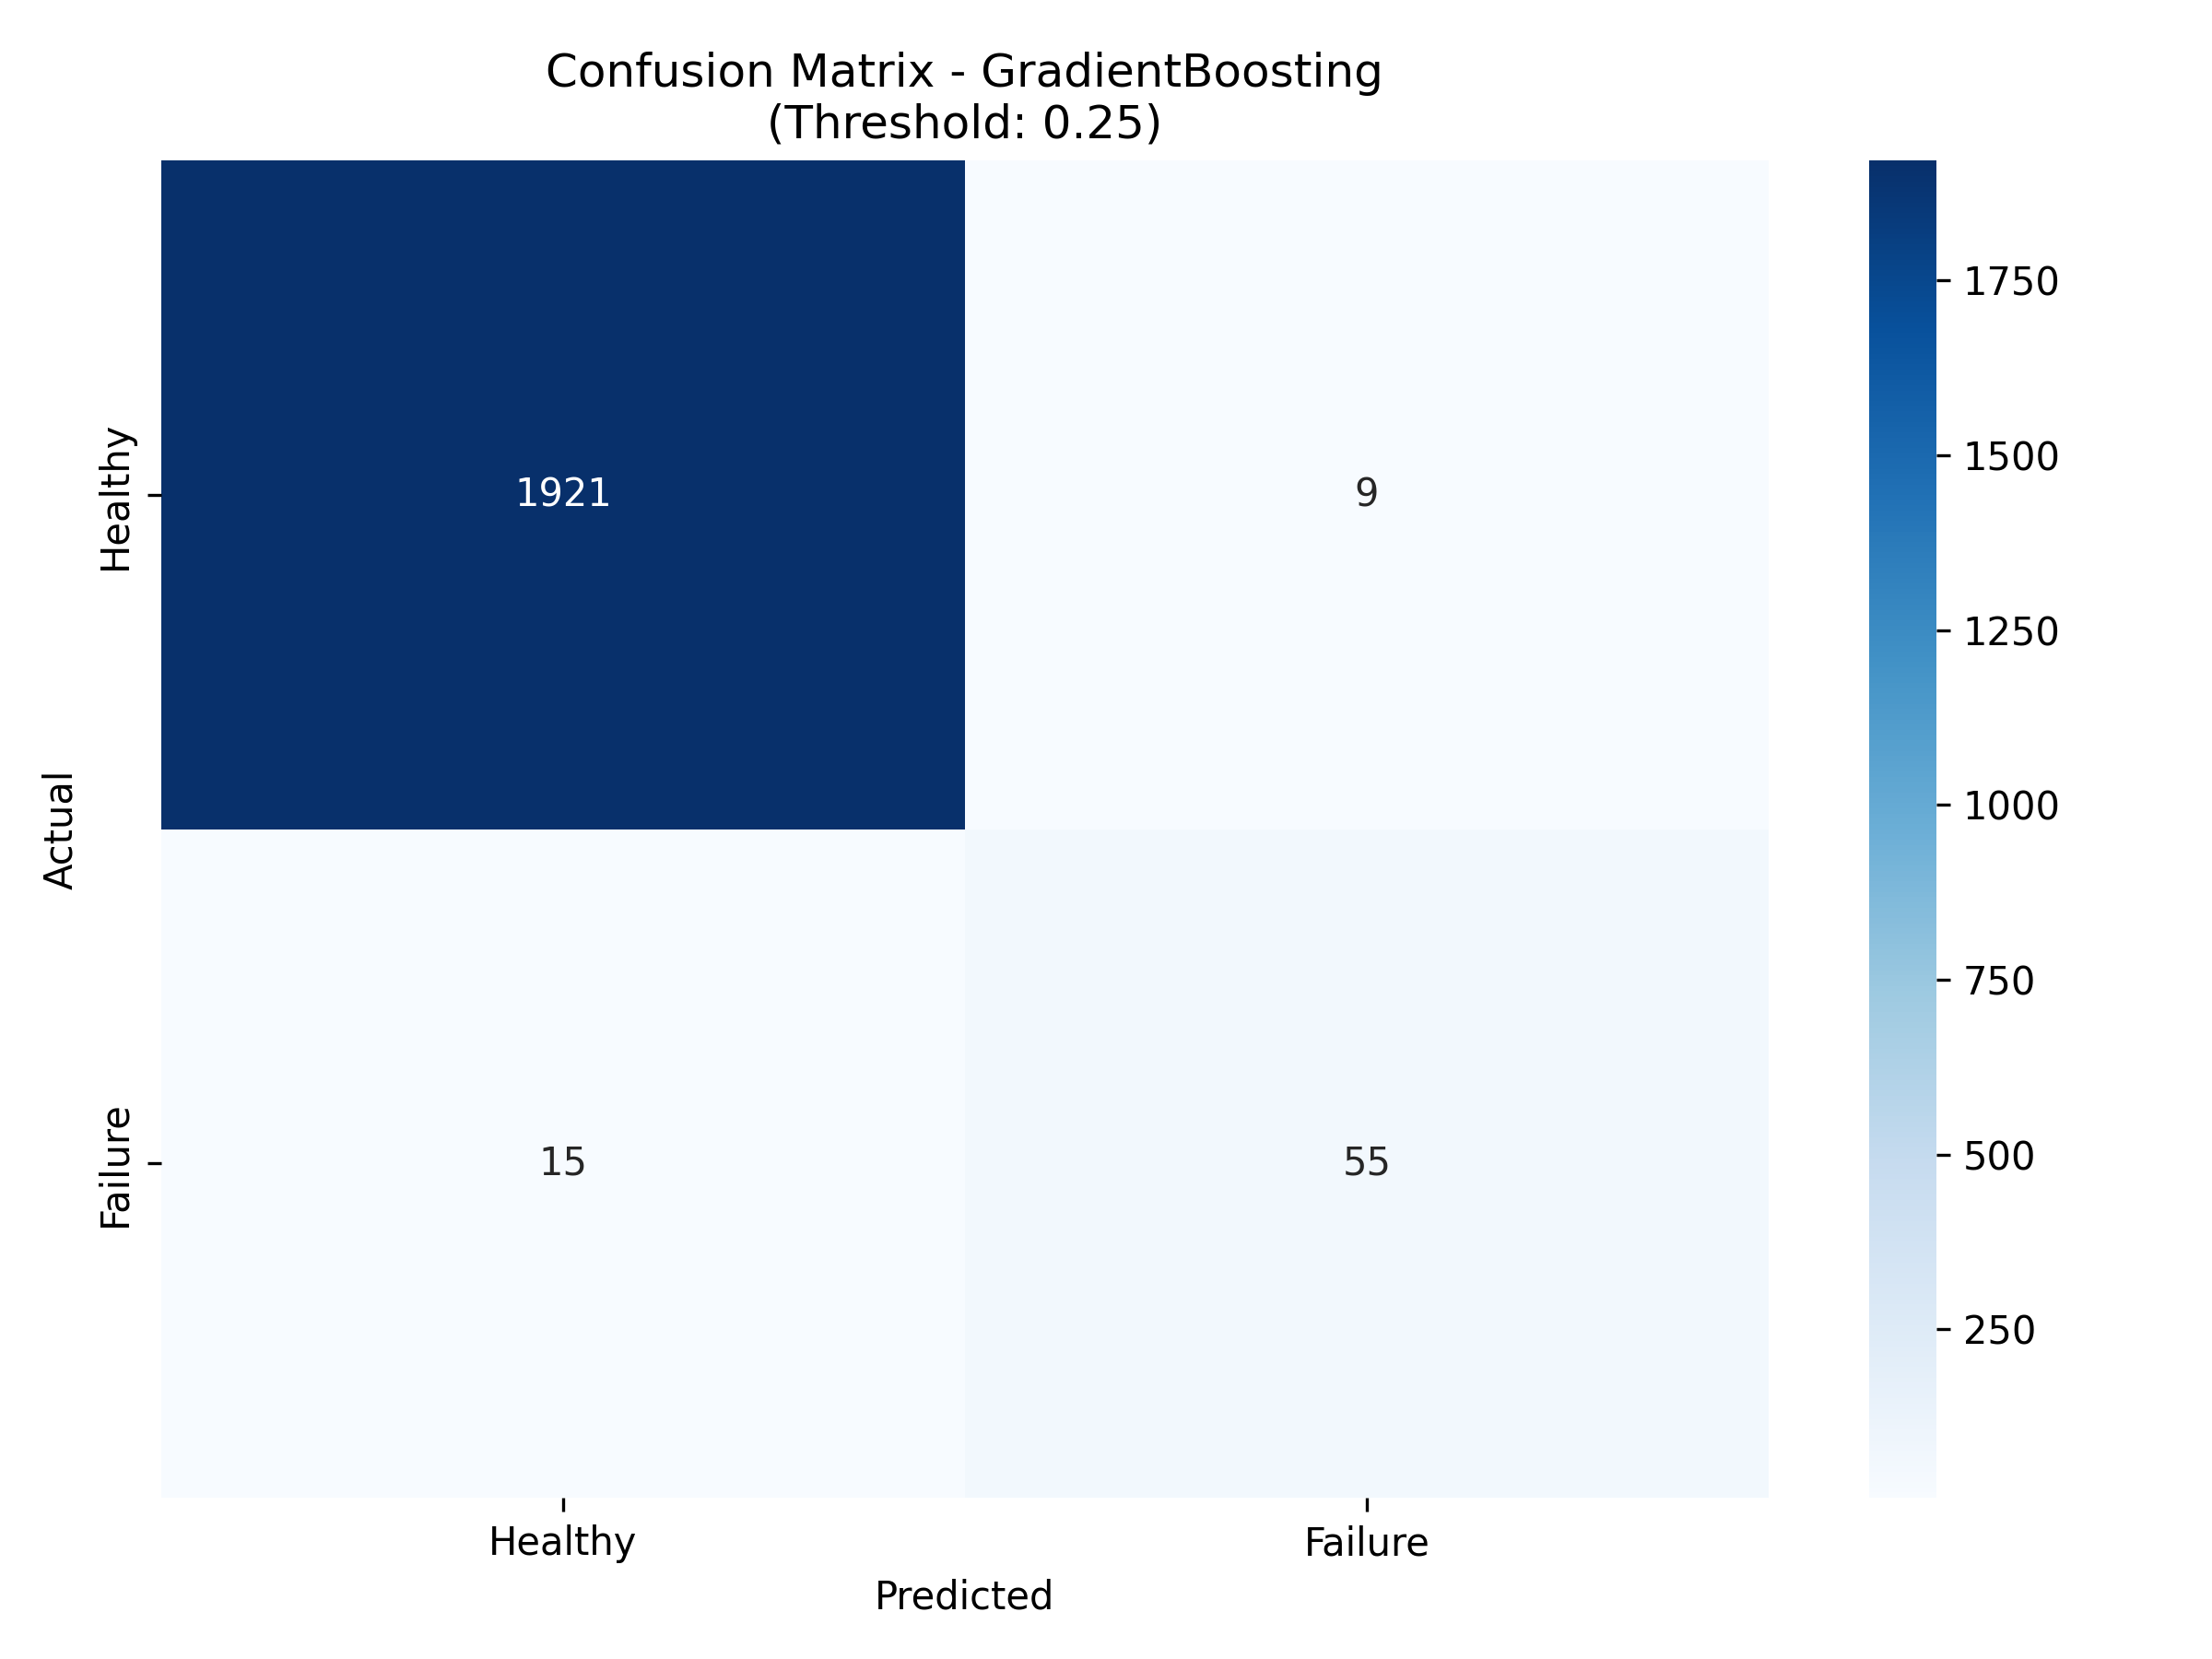
\includegraphics[width=0.74\textwidth]{assets/confusion_matrix.png}
    \caption{Matrice de confusion générée.}
\end{figure}

Le modèle déclenche 64 alertes sur 2 000 cas de test. Parmi ces alertes, 55 correspondent à de vraies pannes et 9 sont des fausses alertes. Il manque 15 pannes. Cette lecture opérationnelle est plus utile que l'accuracy brute.

\section{Courbe ROC et importance des variables}
\begin{figure}[H]
    \centering
    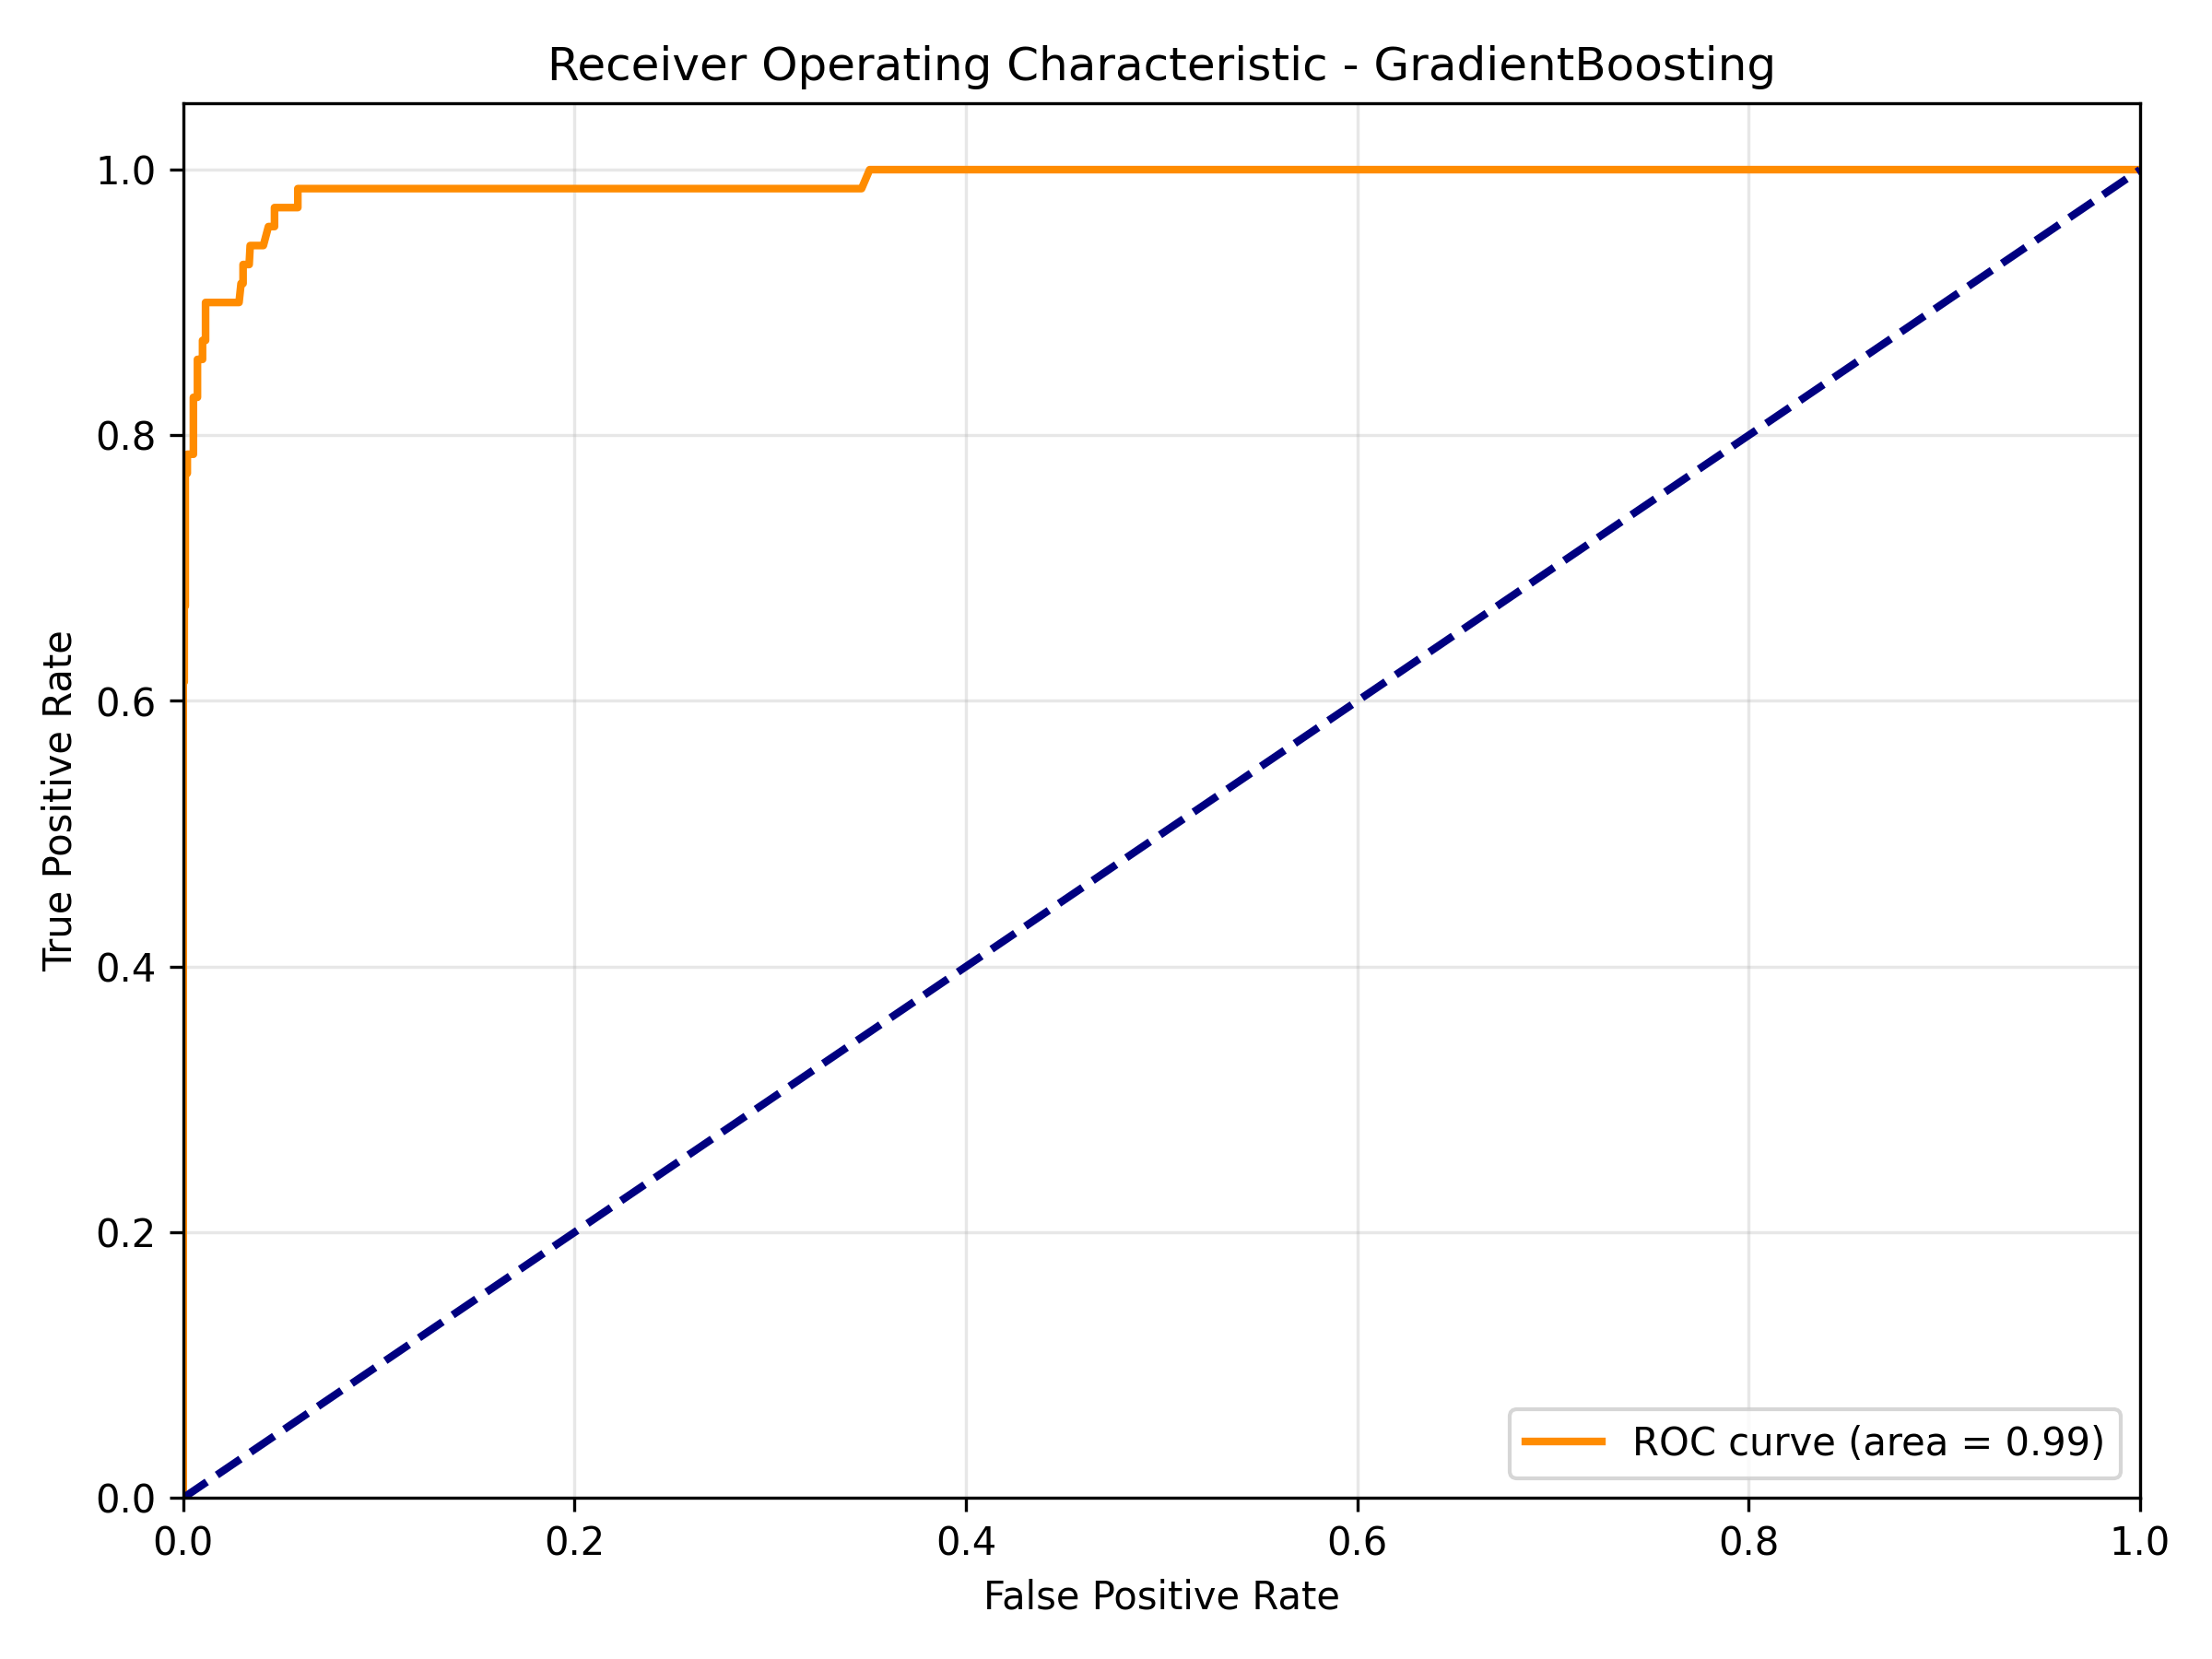
\includegraphics[width=0.82\textwidth]{assets/roc_curve.png}
    \caption{Courbe ROC du modèle actif.}
\end{figure}

\begin{figure}[H]
    \centering
    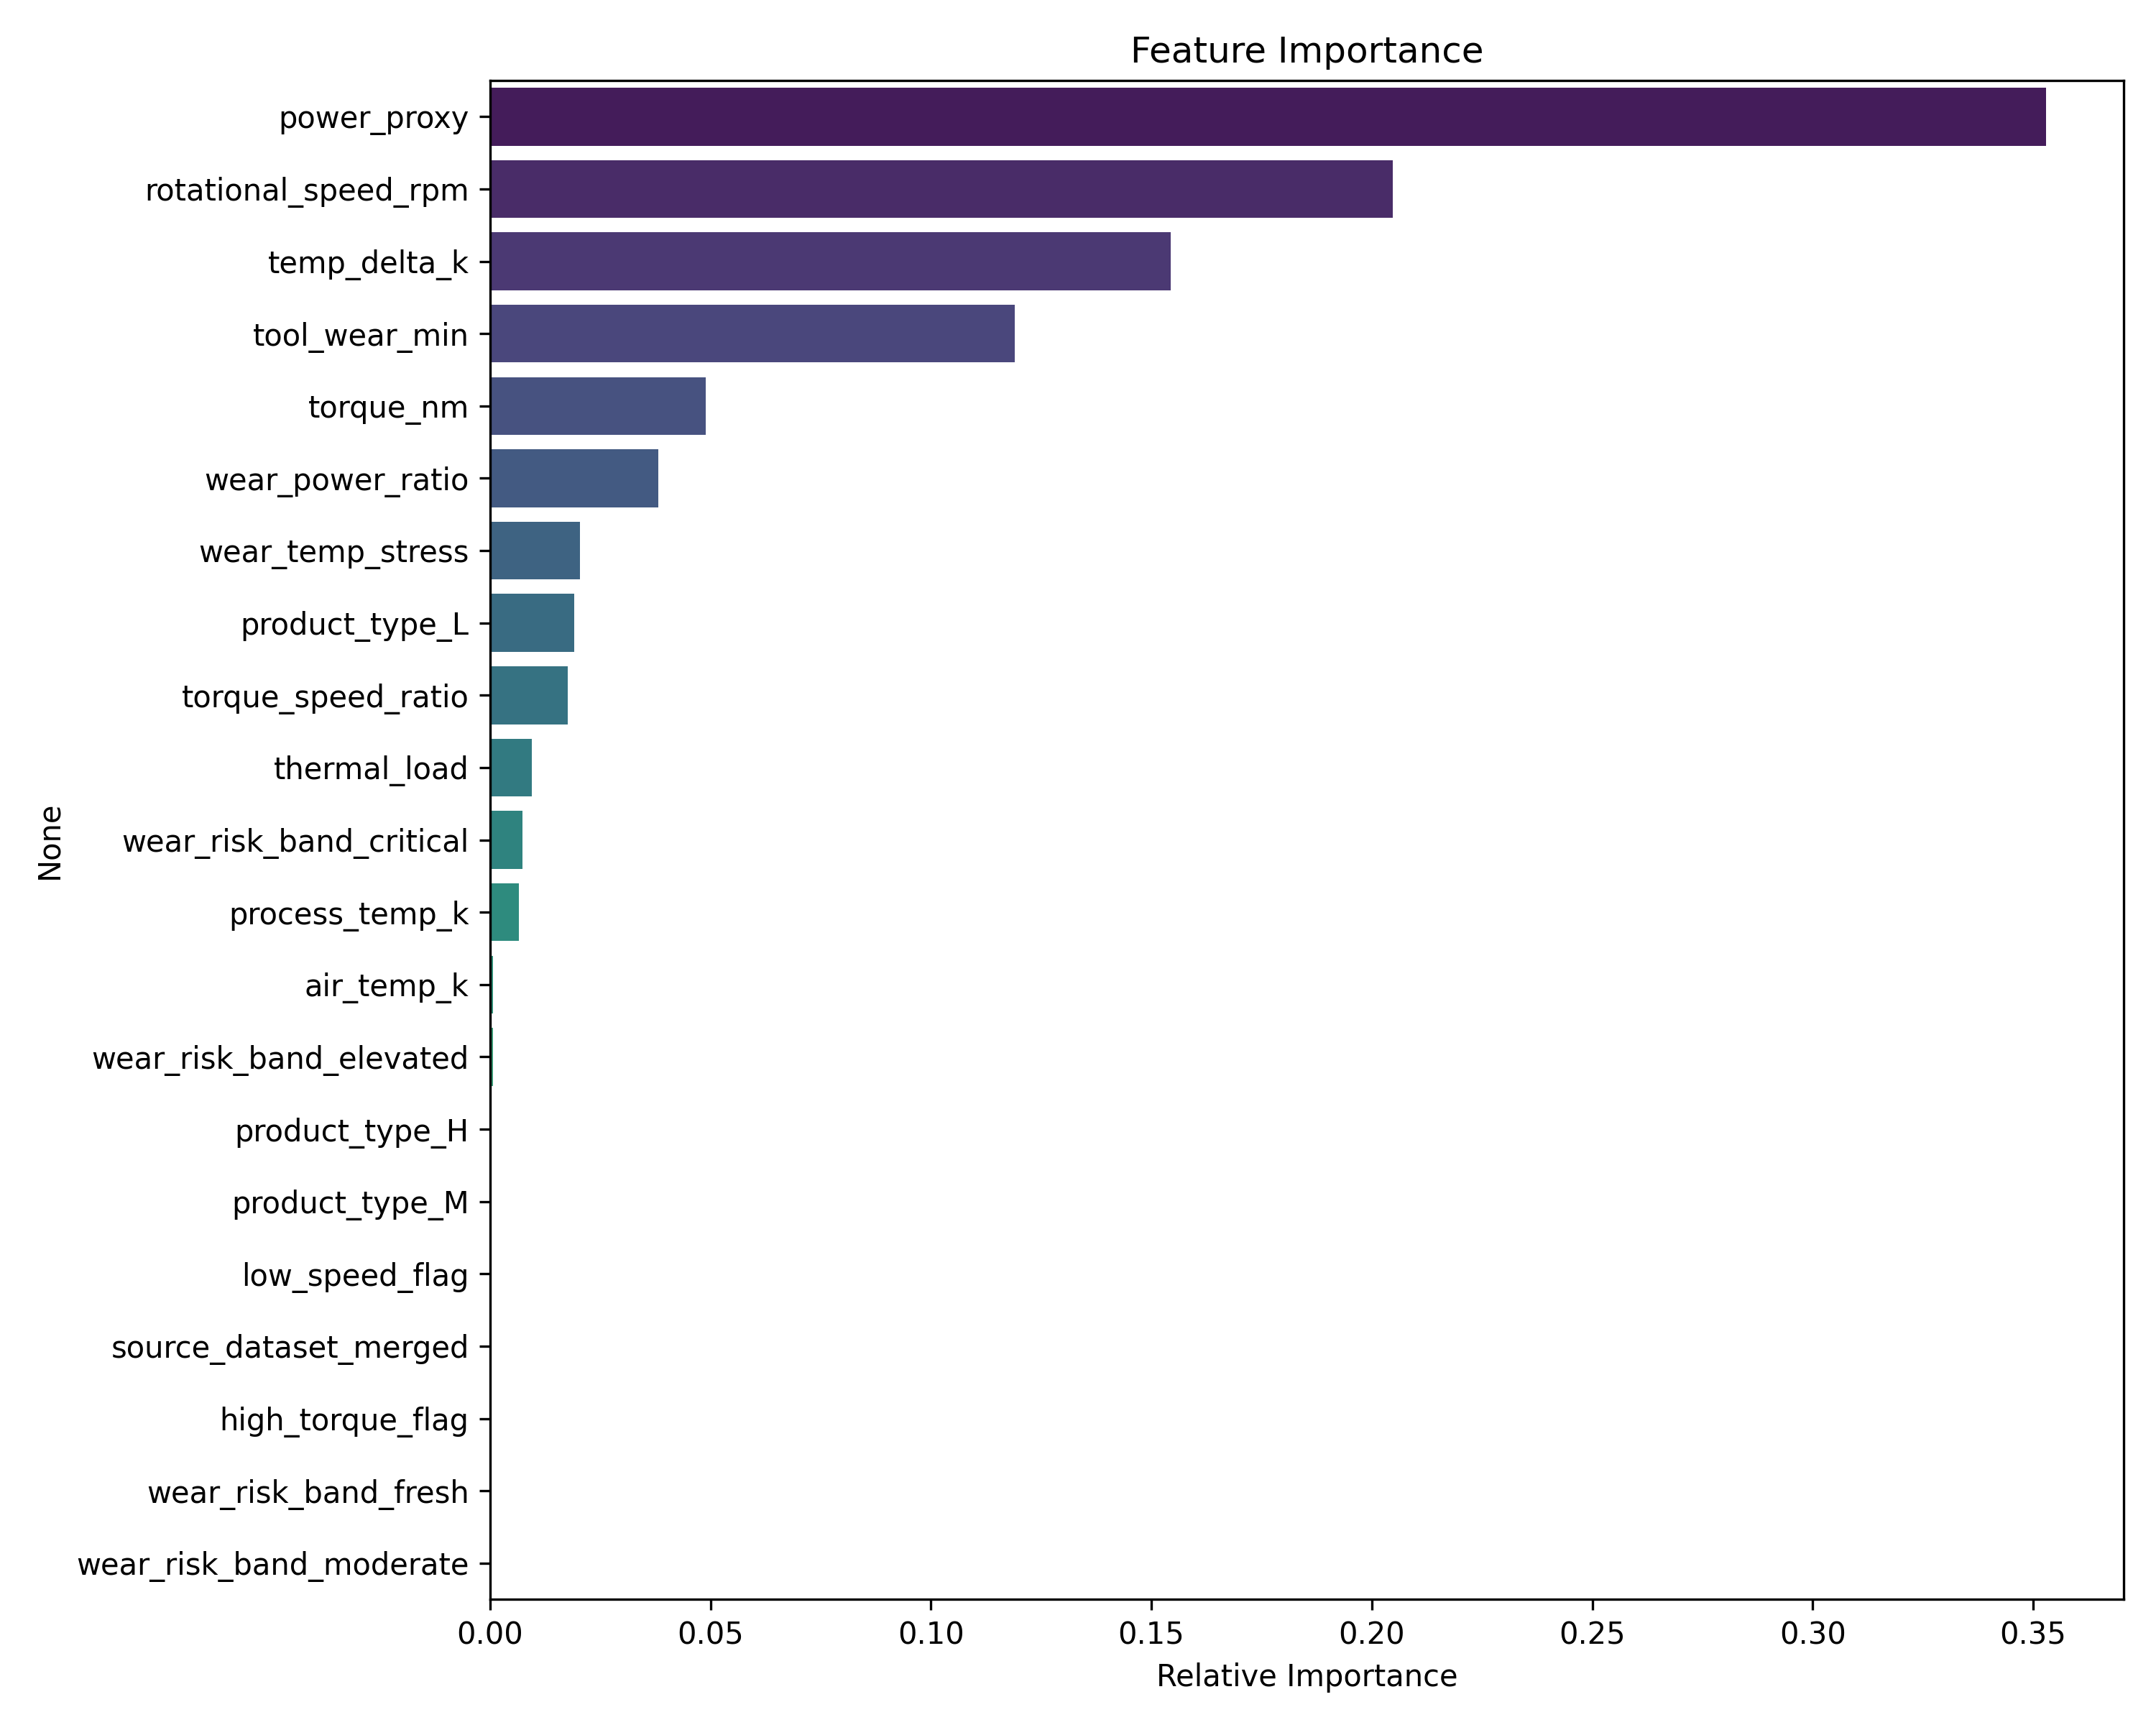
\includegraphics[width=0.82\textwidth]{assets/feature_importance.png}
    \caption{Importance des variables.}
\end{figure}

La ROC AUC élevée montre que le modèle classe très bien les cas risqués. L'importance des variables permet d'expliquer les alertes aux utilisateurs.

\chapter{API, Frontend et Synchronisation}

\section{API FastAPI}
Le backend expose les routes principales : \texttt{/}, \texttt{/notebook}, \texttt{/presentation}, \texttt{/report}, \texttt{/model\_summary}, \texttt{/dashboard}, \texttt{/api/models} et \texttt{/predict}. La route \texttt{/predict} reçoit les valeurs machine, reconstruit les variables d'ingénierie, charge le modèle actif et retourne la probabilité, le seuil, le modèle, la bande de risque et l'action recommandée.

\section{Logique de prédiction}
\begin{lstlisting}[language=Python,caption={Reconstruction simplifiée des variables côté API.}]
row["temp_delta_k"] = row["process_temp_k"] - row["air_temp_k"]
row["power_proxy"] = row["rotational_speed_rpm"] * row["torque_nm"]
row["thermal_load"] = row["temp_delta_k"] * row["torque_nm"]
row["high_torque_flag"] = int(row["torque_nm"] >= 55)
row["low_speed_flag"] = int(row["rotational_speed_rpm"] <= 1400)
\end{lstlisting}

\section{Frontend}
Le dashboard principal met le résultat en avant : probabilité de panne, niveau de risque, seuil, modèle et action. Le ML Lab conserve le contenu technique et les cellules exécutables, mais affiche les mêmes métriques que le dashboard. La présentation raconte le projet de manière courte. La page rapport intègre ce PDF.

\section{Synchronisation}
Toutes les vues utilisent les mêmes exports API : modèle actif GradientBoosting, seuil 0.25, balanced accuracy 89.05\%, pannes capturées 78.57\% et taux d'alerte 3.20\%. Cette synchronisation évite les contradictions entre le dashboard, le ML Lab et la présentation.

\chapter{Déploiement Railway}

\section{Préparation}
Le projet est préparé pour Railway avec \texttt{railway.json} et \texttt{nixpacks.toml}. Railway utilise Python 3.11, installe les dépendances depuis \texttt{api/requirements.txt} et démarre le service avec Uvicorn.

\begin{lstlisting}[language=bash,caption={Commande de démarrage Railway.}]
uvicorn api.app:app --host 0.0.0.0 --port $PORT
\end{lstlisting}

La route \texttt{/health} sert de healthcheck. Le fichier \texttt{.gitignore} et le fichier \texttt{.railwayignore} excluent les fichiers inutiles au déploiement : compilateur LaTeX local, anciens PDF, caches Python et artifacts candidats volumineux.

\section{Contenu déployé}
Le déploiement conserve uniquement le nécessaire pour l'application : backend, frontend, exports JSON, rapport PDF, assets, données utiles au ML Lab et modèle actif GradientBoosting. Cela réduit la taille du projet et accélère l'upload Railway.

\section{Commande CLI}
Le déploiement s'effectue via Railway CLI avec un projet lié et un service web :
\begin{lstlisting}[language=bash]
railway up --detach
\end{lstlisting}

\chapter{Conclusion}
Le projet fournit un workflow complet de maintenance prédictive : données brutes, nettoyage, feature engineering, entraînement, évaluation, API, frontend et rapport. Le résultat final est un outil compréhensible : l'utilisateur saisit les conditions d'une machine, obtient une probabilité de panne et reçoit une action claire.

Le choix de GradientBoosting est justifié par sa performance sur des données tabulaires déséquilibrées. La politique de seuil transforme le modèle en décision opérationnelle. Le frontend synchronisé rend le système plus cohérent et plus simple à utiliser. Le déploiement Railway rend l'application accessible comme service web.

\end{document}
